\documentclass[10pt,tikz,border=5pt]{standalone}
\usepackage[T1]{fontenc}
\usepackage{lmodern,amsmath,booktabs,array,tabularx,microtype,tikz}
\usetikzlibrary{patterns,patterns.meta,shapes.geometric,arrows.meta,calc,positioning}
\begin{document}
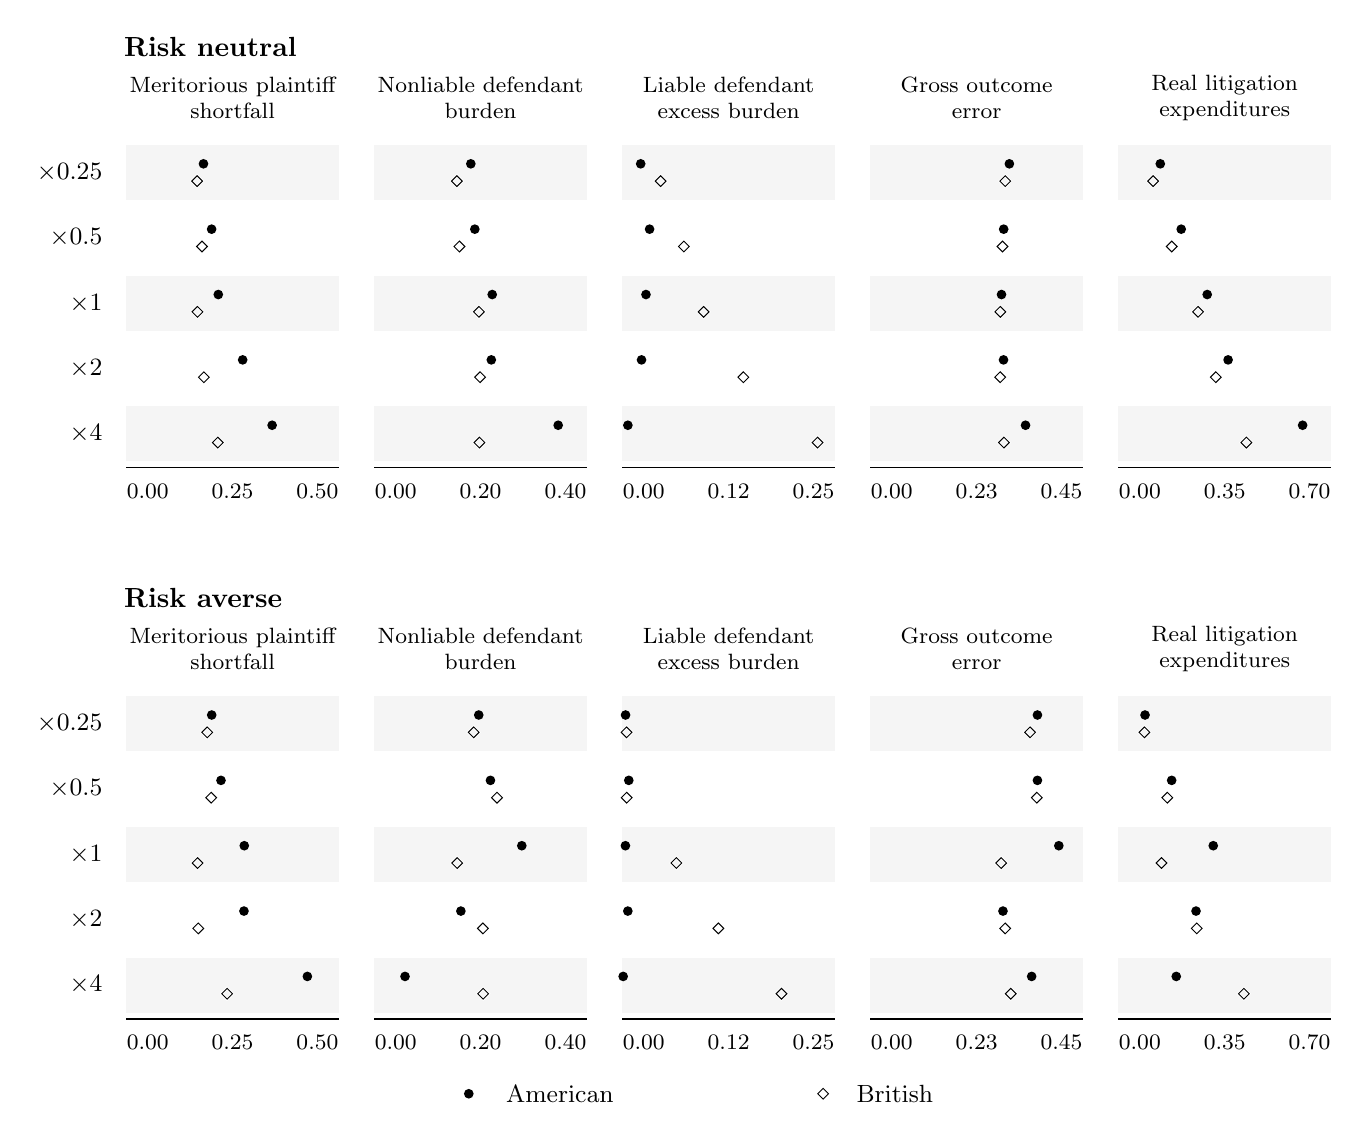
\begin{tikzpicture}[font=\small]
\node[anchor=west,font=\bfseries] at (1.0,13.6) {Risk neutral};
\node[align=center,font=\footnotesize] at (2.5,12.95) {Meritorious plaintiff\\shortfall};
\node[anchor=east] at (0.97,12.0) {$\times 0.25$};
\fill[black!4] (1.15,11.65) rectangle (3.85,12.35);
\begin{scope}[shift={(2.04979650,11.89000000)}]\draw[draw=black,line width=0.350000000pt,line join=miter,miter limit=10,preaction={draw=white,line width=1.000000000pt,line join=miter}] (0pt,1.945812367pt)--(1.945812367pt,0pt)--(0pt,-1.945812367pt)--(-1.945812367pt,0pt)--cycle;\end{scope}
\begin{scope}[shift={(2.13062104,12.11000000)}]\fill[black] (0pt,0pt) circle[radius=1.750000000pt];\end{scope}
\node[anchor=east] at (0.97,11.17) {$\times 0.5$};
\fill[black!0] (1.15,10.82) rectangle (3.85,11.52);
\begin{scope}[shift={(2.11233160,11.06000000)}]\draw[draw=black,line width=0.350000000pt,line join=miter,miter limit=10,preaction={draw=white,line width=1.000000000pt,line join=miter}] (0pt,1.945812367pt)--(1.945812367pt,0pt)--(0pt,-1.945812367pt)--(-1.945812367pt,0pt)--cycle;\end{scope}
\begin{scope}[shift={(2.23392036,11.28000000)}]\fill[black] (0pt,0pt) circle[radius=1.750000000pt];\end{scope}
\node[anchor=east] at (0.97,10.34) {$\times 1$};
\fill[black!4] (1.15,9.99) rectangle (3.85,10.69);
\begin{scope}[shift={(2.05411881,10.23000000)}]\draw[draw=black,line width=0.350000000pt,line join=miter,miter limit=10,preaction={draw=white,line width=1.000000000pt,line join=miter}] (0pt,1.945812367pt)--(1.945812367pt,0pt)--(0pt,-1.945812367pt)--(-1.945812367pt,0pt)--cycle;\end{scope}
\begin{scope}[shift={(2.31875792,10.45000000)}]\fill[black] (0pt,0pt) circle[radius=1.750000000pt];\end{scope}
\node[anchor=east] at (0.97,9.51) {$\times 2$};
\fill[black!0] (1.15,9.16) rectangle (3.85,9.86);
\begin{scope}[shift={(2.13553751,9.40000000)}]\draw[draw=black,line width=0.350000000pt,line join=miter,miter limit=10,preaction={draw=white,line width=1.000000000pt,line join=miter}] (0pt,1.945812367pt)--(1.945812367pt,0pt)--(0pt,-1.945812367pt)--(-1.945812367pt,0pt)--cycle;\end{scope}
\begin{scope}[shift={(2.62835517,9.62000000)}]\fill[black] (0pt,0pt) circle[radius=1.750000000pt];\end{scope}
\node[anchor=east] at (0.97,8.68) {$\times 4$};
\fill[black!4] (1.15,8.33) rectangle (3.85,9.03);
\begin{scope}[shift={(2.31256619,8.57000000)}]\draw[draw=black,line width=0.350000000pt,line join=miter,miter limit=10,preaction={draw=white,line width=1.000000000pt,line join=miter}] (0pt,1.945812367pt)--(1.945812367pt,0pt)--(0pt,-1.945812367pt)--(-1.945812367pt,0pt)--cycle;\end{scope}
\begin{scope}[shift={(3.00234385,8.79000000)}]\fill[black] (0pt,0pt) circle[radius=1.750000000pt];\end{scope}
\draw (1.15,8.25)--(3.85,8.25);
\node[anchor=north west,font=\footnotesize,inner xsep=0pt] at (1.15,8.17) {0.00};
\node[anchor=north,font=\footnotesize,inner xsep=0pt] at (2.5,8.17) {0.25};
\node[anchor=north east,font=\footnotesize,inner xsep=0pt] at (3.85,8.17) {0.50};
\node[align=center,font=\footnotesize] at (5.65,12.95) {Nonliable defendant\\burden};
\fill[black!4] (4.3,11.65) rectangle (7.0,12.35);
\begin{scope}[shift={(5.34897541,11.89000000)}]\draw[draw=black,line width=0.350000000pt,line join=miter,miter limit=10,preaction={draw=white,line width=1.000000000pt,line join=miter}] (0pt,1.945812367pt)--(1.945812367pt,0pt)--(0pt,-1.945812367pt)--(-1.945812367pt,0pt)--cycle;\end{scope}
\begin{scope}[shift={(5.52574351,12.11000000)}]\fill[black] (0pt,0pt) circle[radius=1.750000000pt];\end{scope}
\fill[black!0] (4.3,10.82) rectangle (7.0,11.52);
\begin{scope}[shift={(5.38119670,11.06000000)}]\draw[draw=black,line width=0.350000000pt,line join=miter,miter limit=10,preaction={draw=white,line width=1.000000000pt,line join=miter}] (0pt,1.945812367pt)--(1.945812367pt,0pt)--(0pt,-1.945812367pt)--(-1.945812367pt,0pt)--cycle;\end{scope}
\begin{scope}[shift={(5.57651970,11.28000000)}]\fill[black] (0pt,0pt) circle[radius=1.750000000pt];\end{scope}
\fill[black!4] (4.3,9.99) rectangle (7.0,10.69);
\begin{scope}[shift={(5.62877614,10.23000000)}]\draw[draw=black,line width=0.350000000pt,line join=miter,miter limit=10,preaction={draw=white,line width=1.000000000pt,line join=miter}] (0pt,1.945812367pt)--(1.945812367pt,0pt)--(0pt,-1.945812367pt)--(-1.945812367pt,0pt)--cycle;\end{scope}
\begin{scope}[shift={(5.79762348,10.45000000)}]\fill[black] (0pt,0pt) circle[radius=1.750000000pt];\end{scope}
\fill[black!0] (4.3,9.16) rectangle (7.0,9.86);
\begin{scope}[shift={(5.64330954,9.40000000)}]\draw[draw=black,line width=0.350000000pt,line join=miter,miter limit=10,preaction={draw=white,line width=1.000000000pt,line join=miter}] (0pt,1.945812367pt)--(1.945812367pt,0pt)--(0pt,-1.945812367pt)--(-1.945812367pt,0pt)--cycle;\end{scope}
\begin{scope}[shift={(5.78616676,9.62000000)}]\fill[black] (0pt,0pt) circle[radius=1.750000000pt];\end{scope}
\fill[black!4] (4.3,8.33) rectangle (7.0,9.03);
\begin{scope}[shift={(5.63496128,8.57000000)}]\draw[draw=black,line width=0.350000000pt,line join=miter,miter limit=10,preaction={draw=white,line width=1.000000000pt,line join=miter}] (0pt,1.945812367pt)--(1.945812367pt,0pt)--(0pt,-1.945812367pt)--(-1.945812367pt,0pt)--cycle;\end{scope}
\begin{scope}[shift={(6.63541167,8.79000000)}]\fill[black] (0pt,0pt) circle[radius=1.750000000pt];\end{scope}
\draw (4.3,8.25)--(7.0,8.25);
\node[anchor=north west,font=\footnotesize,inner xsep=0pt] at (4.3,8.17) {0.00};
\node[anchor=north,font=\footnotesize,inner xsep=0pt] at (5.65,8.17) {0.20};
\node[anchor=north east,font=\footnotesize,inner xsep=0pt] at (7.0,8.17) {0.40};
\node[align=center,font=\footnotesize] at (8.799999999999999,12.95) {Liable defendant\\excess burden};
\fill[black!4] (7.449999999999999,11.65) rectangle (10.149999999999999,12.35);
\begin{scope}[shift={(7.93629639,11.89000000)}]\draw[draw=black,line width=0.350000000pt,line join=miter,miter limit=10,preaction={draw=white,line width=1.000000000pt,line join=miter}] (0pt,1.945812367pt)--(1.945812367pt,0pt)--(0pt,-1.945812367pt)--(-1.945812367pt,0pt)--cycle;\end{scope}
\begin{scope}[shift={(7.68318178,12.11000000)}]\fill[black] (0pt,0pt) circle[radius=1.750000000pt];\end{scope}
\fill[black!0] (7.449999999999999,10.82) rectangle (10.149999999999999,11.52);
\begin{scope}[shift={(8.23187516,11.06000000)}]\draw[draw=black,line width=0.350000000pt,line join=miter,miter limit=10,preaction={draw=white,line width=1.000000000pt,line join=miter}] (0pt,1.945812367pt)--(1.945812367pt,0pt)--(0pt,-1.945812367pt)--(-1.945812367pt,0pt)--cycle;\end{scope}
\begin{scope}[shift={(7.79620664,11.28000000)}]\fill[black] (0pt,0pt) circle[radius=1.750000000pt];\end{scope}
\fill[black!4] (7.449999999999999,9.99) rectangle (10.149999999999999,10.69);
\begin{scope}[shift={(8.48271391,10.23000000)}]\draw[draw=black,line width=0.350000000pt,line join=miter,miter limit=10,preaction={draw=white,line width=1.000000000pt,line join=miter}] (0pt,1.945812367pt)--(1.945812367pt,0pt)--(0pt,-1.945812367pt)--(-1.945812367pt,0pt)--cycle;\end{scope}
\begin{scope}[shift={(7.75028162,10.45000000)}]\fill[black] (0pt,0pt) circle[radius=1.750000000pt];\end{scope}
\fill[black!0] (7.449999999999999,9.16) rectangle (10.149999999999999,9.86);
\begin{scope}[shift={(8.98692604,9.40000000)}]\draw[draw=black,line width=0.350000000pt,line join=miter,miter limit=10,preaction={draw=white,line width=1.000000000pt,line join=miter}] (0pt,1.945812367pt)--(1.945812367pt,0pt)--(0pt,-1.945812367pt)--(-1.945812367pt,0pt)--cycle;\end{scope}
\begin{scope}[shift={(7.69368095,9.62000000)}]\fill[black] (0pt,0pt) circle[radius=1.750000000pt];\end{scope}
\fill[black!4] (7.449999999999999,8.33) rectangle (10.149999999999999,9.03);
\begin{scope}[shift={(9.92881009,8.57000000)}]\draw[draw=black,line width=0.350000000pt,line join=miter,miter limit=10,preaction={draw=white,line width=1.000000000pt,line join=miter}] (0pt,1.945812367pt)--(1.945812367pt,0pt)--(0pt,-1.945812367pt)--(-1.945812367pt,0pt)--cycle;\end{scope}
\begin{scope}[shift={(7.52036142,8.79000000)}]\fill[black] (0pt,0pt) circle[radius=1.750000000pt];\end{scope}
\draw (7.449999999999999,8.25)--(10.149999999999999,8.25);
\node[anchor=north west,font=\footnotesize,inner xsep=0pt] at (7.449999999999999,8.17) {0.00};
\node[anchor=north,font=\footnotesize,inner xsep=0pt] at (8.799999999999999,8.17) {0.12};
\node[anchor=north east,font=\footnotesize,inner xsep=0pt] at (10.149999999999999,8.17) {0.25};
\node[align=center,font=\footnotesize] at (11.95,12.95) {Gross outcome\\error};
\fill[black!4] (10.6,11.65) rectangle (13.3,12.35);
\begin{scope}[shift={(12.31296749,11.89000000)}]\draw[draw=black,line width=0.350000000pt,line join=miter,miter limit=10,preaction={draw=white,line width=1.000000000pt,line join=miter}] (0pt,1.945812367pt)--(1.945812367pt,0pt)--(0pt,-1.945812367pt)--(-1.945812367pt,0pt)--cycle;\end{scope}
\begin{scope}[shift={(12.36530625,12.11000000)}]\fill[black] (0pt,0pt) circle[radius=1.750000000pt];\end{scope}
\fill[black!0] (10.6,10.82) rectangle (13.3,11.52);
\begin{scope}[shift={(12.27813181,11.06000000)}]\draw[draw=black,line width=0.350000000pt,line join=miter,miter limit=10,preaction={draw=white,line width=1.000000000pt,line join=miter}] (0pt,1.945812367pt)--(1.945812367pt,0pt)--(0pt,-1.945812367pt)--(-1.945812367pt,0pt)--cycle;\end{scope}
\begin{scope}[shift={(12.29315648,11.28000000)}]\fill[black] (0pt,0pt) circle[radius=1.750000000pt];\end{scope}
\fill[black!4] (10.6,9.99) rectangle (13.3,10.69);
\begin{scope}[shift={(12.25043978,10.23000000)}]\draw[draw=black,line width=0.350000000pt,line join=miter,miter limit=10,preaction={draw=white,line width=1.000000000pt,line join=miter}] (0pt,1.945812367pt)--(1.945812367pt,0pt)--(0pt,-1.945812367pt)--(-1.945812367pt,0pt)--cycle;\end{scope}
\begin{scope}[shift={(12.26538682,10.45000000)}]\fill[black] (0pt,0pt) circle[radius=1.750000000pt];\end{scope}
\fill[black!0] (10.6,9.16) rectangle (13.3,9.86);
\begin{scope}[shift={(12.24875621,9.40000000)}]\draw[draw=black,line width=0.350000000pt,line join=miter,miter limit=10,preaction={draw=white,line width=1.000000000pt,line join=miter}] (0pt,1.945812367pt)--(1.945812367pt,0pt)--(0pt,-1.945812367pt)--(-1.945812367pt,0pt)--cycle;\end{scope}
\begin{scope}[shift={(12.29100360,9.62000000)}]\fill[black] (0pt,0pt) circle[radius=1.750000000pt];\end{scope}
\fill[black!4] (10.6,8.33) rectangle (13.3,9.03);
\begin{scope}[shift={(12.29663193,8.57000000)}]\draw[draw=black,line width=0.350000000pt,line join=miter,miter limit=10,preaction={draw=white,line width=1.000000000pt,line join=miter}] (0pt,1.945812367pt)--(1.945812367pt,0pt)--(0pt,-1.945812367pt)--(-1.945812367pt,0pt)--cycle;\end{scope}
\begin{scope}[shift={(12.57063430,8.79000000)}]\fill[black] (0pt,0pt) circle[radius=1.750000000pt];\end{scope}
\draw (10.6,8.25)--(13.3,8.25);
\node[anchor=north west,font=\footnotesize,inner xsep=0pt] at (10.6,8.17) {0.00};
\node[anchor=north,font=\footnotesize,inner xsep=0pt] at (11.95,8.17) {0.23};
\node[anchor=north east,font=\footnotesize,inner xsep=0pt] at (13.3,8.17) {0.45};
\node[align=center,font=\footnotesize] at (15.1,12.95) {Real litigation\\expenditures};
\fill[black!4] (13.75,11.65) rectangle (16.45,12.35);
\begin{scope}[shift={(14.19078306,11.89000000)}]\draw[draw=black,line width=0.350000000pt,line join=miter,miter limit=10,preaction={draw=white,line width=1.000000000pt,line join=miter}] (0pt,1.945812367pt)--(1.945812367pt,0pt)--(0pt,-1.945812367pt)--(-1.945812367pt,0pt)--cycle;\end{scope}
\begin{scope}[shift={(14.28205747,12.11000000)}]\fill[black] (0pt,0pt) circle[radius=1.750000000pt];\end{scope}
\fill[black!0] (13.75,10.82) rectangle (16.45,11.52);
\begin{scope}[shift={(14.42704365,11.06000000)}]\draw[draw=black,line width=0.350000000pt,line join=miter,miter limit=10,preaction={draw=white,line width=1.000000000pt,line join=miter}] (0pt,1.945812367pt)--(1.945812367pt,0pt)--(0pt,-1.945812367pt)--(-1.945812367pt,0pt)--cycle;\end{scope}
\begin{scope}[shift={(14.54772975,11.28000000)}]\fill[black] (0pt,0pt) circle[radius=1.750000000pt];\end{scope}
\fill[black!4] (13.75,9.99) rectangle (16.45,10.69);
\begin{scope}[shift={(14.76167432,10.23000000)}]\draw[draw=black,line width=0.350000000pt,line join=miter,miter limit=10,preaction={draw=white,line width=1.000000000pt,line join=miter}] (0pt,1.945812367pt)--(1.945812367pt,0pt)--(0pt,-1.945812367pt)--(-1.945812367pt,0pt)--cycle;\end{scope}
\begin{scope}[shift={(14.87784958,10.45000000)}]\fill[black] (0pt,0pt) circle[radius=1.750000000pt];\end{scope}
\fill[black!0] (13.75,9.16) rectangle (16.45,9.86);
\begin{scope}[shift={(14.98666021,9.40000000)}]\draw[draw=black,line width=0.350000000pt,line join=miter,miter limit=10,preaction={draw=white,line width=1.000000000pt,line join=miter}] (0pt,1.945812367pt)--(1.945812367pt,0pt)--(0pt,-1.945812367pt)--(-1.945812367pt,0pt)--cycle;\end{scope}
\begin{scope}[shift={(15.14316451,9.62000000)}]\fill[black] (0pt,0pt) circle[radius=1.750000000pt];\end{scope}
\fill[black!4] (13.75,8.33) rectangle (16.45,9.03);
\begin{scope}[shift={(15.37521054,8.57000000)}]\draw[draw=black,line width=0.350000000pt,line join=miter,miter limit=10,preaction={draw=white,line width=1.000000000pt,line join=miter}] (0pt,1.945812367pt)--(1.945812367pt,0pt)--(0pt,-1.945812367pt)--(-1.945812367pt,0pt)--cycle;\end{scope}
\begin{scope}[shift={(16.08963496,8.79000000)}]\fill[black] (0pt,0pt) circle[radius=1.750000000pt];\end{scope}
\draw (13.75,8.25)--(16.45,8.25);
\node[anchor=north west,font=\footnotesize,inner xsep=0pt] at (13.75,8.17) {0.00};
\node[anchor=north,font=\footnotesize,inner xsep=0pt] at (15.1,8.17) {0.35};
\node[anchor=north east,font=\footnotesize,inner xsep=0pt] at (16.45,8.17) {0.70};
\node[anchor=west,font=\bfseries] at (1.0,6.6) {Risk averse};
\node[align=center,font=\footnotesize] at (2.5,5.95) {Meritorious plaintiff\\shortfall};
\node[anchor=east] at (0.97,5.0) {$\times 0.25$};
\fill[black!4] (1.15,4.65) rectangle (3.85,5.35);
\begin{scope}[shift={(2.17822415,4.89000000)}]\draw[draw=black,line width=0.350000000pt,line join=miter,miter limit=10,preaction={draw=white,line width=1.000000000pt,line join=miter}] (0pt,1.945812367pt)--(1.945812367pt,0pt)--(0pt,-1.945812367pt)--(-1.945812367pt,0pt)--cycle;\end{scope}
\begin{scope}[shift={(2.23507581,5.11000000)}]\fill[black] (0pt,0pt) circle[radius=1.750000000pt];\end{scope}
\node[anchor=east] at (0.97,4.17) {$\times 0.5$};
\fill[black!0] (1.15,3.82) rectangle (3.85,4.52);
\begin{scope}[shift={(2.22881870,4.06000000)}]\draw[draw=black,line width=0.350000000pt,line join=miter,miter limit=10,preaction={draw=white,line width=1.000000000pt,line join=miter}] (0pt,1.945812367pt)--(1.945812367pt,0pt)--(0pt,-1.945812367pt)--(-1.945812367pt,0pt)--cycle;\end{scope}
\begin{scope}[shift={(2.35293843,4.28000000)}]\fill[black] (0pt,0pt) circle[radius=1.750000000pt];\end{scope}
\node[anchor=east] at (0.97,3.34) {$\times 1$};
\fill[black!4] (1.15,2.9899999999999998) rectangle (3.85,3.69);
\begin{scope}[shift={(2.05564880,3.23000000)}]\draw[draw=black,line width=0.350000000pt,line join=miter,miter limit=10,preaction={draw=white,line width=1.000000000pt,line join=miter}] (0pt,1.945812367pt)--(1.945812367pt,0pt)--(0pt,-1.945812367pt)--(-1.945812367pt,0pt)--cycle;\end{scope}
\begin{scope}[shift={(2.64866079,3.45000000)}]\fill[black] (0pt,0pt) circle[radius=1.750000000pt];\end{scope}
\node[anchor=east] at (0.97,2.5100000000000002) {$\times 2$};
\fill[black!0] (1.15,2.16) rectangle (3.85,2.8600000000000003);
\begin{scope}[shift={(2.06482488,2.40000000)}]\draw[draw=black,line width=0.350000000pt,line join=miter,miter limit=10,preaction={draw=white,line width=1.000000000pt,line join=miter}] (0pt,1.945812367pt)--(1.945812367pt,0pt)--(0pt,-1.945812367pt)--(-1.945812367pt,0pt)--cycle;\end{scope}
\begin{scope}[shift={(2.64465622,2.62000000)}]\fill[black] (0pt,0pt) circle[radius=1.750000000pt];\end{scope}
\node[anchor=east] at (0.97,1.6800000000000002) {$\times 4$};
\fill[black!4] (1.15,1.33) rectangle (3.85,2.0300000000000002);
\begin{scope}[shift={(2.43030274,1.57000000)}]\draw[draw=black,line width=0.350000000pt,line join=miter,miter limit=10,preaction={draw=white,line width=1.000000000pt,line join=miter}] (0pt,1.945812367pt)--(1.945812367pt,0pt)--(0pt,-1.945812367pt)--(-1.945812367pt,0pt)--cycle;\end{scope}
\begin{scope}[shift={(3.44983946,1.79000000)}]\fill[black] (0pt,0pt) circle[radius=1.750000000pt];\end{scope}
\draw (1.15,1.25)--(3.85,1.25);
\node[anchor=north west,font=\footnotesize,inner xsep=0pt] at (1.15,1.17) {0.00};
\node[anchor=north,font=\footnotesize,inner xsep=0pt] at (2.5,1.17) {0.25};
\node[anchor=north east,font=\footnotesize,inner xsep=0pt] at (3.85,1.17) {0.50};
\node[align=center,font=\footnotesize] at (5.65,5.95) {Nonliable defendant\\burden};
\fill[black!4] (4.3,4.65) rectangle (7.0,5.35);
\begin{scope}[shift={(5.56175473,4.89000000)}]\draw[draw=black,line width=0.350000000pt,line join=miter,miter limit=10,preaction={draw=white,line width=1.000000000pt,line join=miter}] (0pt,1.945812367pt)--(1.945812367pt,0pt)--(0pt,-1.945812367pt)--(-1.945812367pt,0pt)--cycle;\end{scope}
\begin{scope}[shift={(5.62651932,5.11000000)}]\fill[black] (0pt,0pt) circle[radius=1.750000000pt];\end{scope}
\fill[black!0] (4.3,3.82) rectangle (7.0,4.52);
\begin{scope}[shift={(5.85824291,4.06000000)}]\draw[draw=black,line width=0.350000000pt,line join=miter,miter limit=10,preaction={draw=white,line width=1.000000000pt,line join=miter}] (0pt,1.945812367pt)--(1.945812367pt,0pt)--(0pt,-1.945812367pt)--(-1.945812367pt,0pt)--cycle;\end{scope}
\begin{scope}[shift={(5.77510891,4.28000000)}]\fill[black] (0pt,0pt) circle[radius=1.750000000pt];\end{scope}
\fill[black!4] (4.3,2.9899999999999998) rectangle (7.0,3.69);
\begin{scope}[shift={(5.35268463,3.23000000)}]\draw[draw=black,line width=0.350000000pt,line join=miter,miter limit=10,preaction={draw=white,line width=1.000000000pt,line join=miter}] (0pt,1.945812367pt)--(1.945812367pt,0pt)--(0pt,-1.945812367pt)--(-1.945812367pt,0pt)--cycle;\end{scope}
\begin{scope}[shift={(6.17330595,3.45000000)}]\fill[black] (0pt,0pt) circle[radius=1.750000000pt];\end{scope}
\fill[black!0] (4.3,2.16) rectangle (7.0,2.8600000000000003);
\begin{scope}[shift={(5.67942197,2.40000000)}]\draw[draw=black,line width=0.350000000pt,line join=miter,miter limit=10,preaction={draw=white,line width=1.000000000pt,line join=miter}] (0pt,1.945812367pt)--(1.945812367pt,0pt)--(0pt,-1.945812367pt)--(-1.945812367pt,0pt)--cycle;\end{scope}
\begin{scope}[shift={(5.39958674,2.62000000)}]\fill[black] (0pt,0pt) circle[radius=1.750000000pt];\end{scope}
\fill[black!4] (4.3,1.33) rectangle (7.0,2.0300000000000002);
\begin{scope}[shift={(5.68265150,1.57000000)}]\draw[draw=black,line width=0.350000000pt,line join=miter,miter limit=10,preaction={draw=white,line width=1.000000000pt,line join=miter}] (0pt,1.945812367pt)--(1.945812367pt,0pt)--(0pt,-1.945812367pt)--(-1.945812367pt,0pt)--cycle;\end{scope}
\begin{scope}[shift={(4.69028333,1.79000000)}]\fill[black] (0pt,0pt) circle[radius=1.750000000pt];\end{scope}
\draw (4.3,1.25)--(7.0,1.25);
\node[anchor=north west,font=\footnotesize,inner xsep=0pt] at (4.3,1.17) {0.00};
\node[anchor=north,font=\footnotesize,inner xsep=0pt] at (5.65,1.17) {0.20};
\node[anchor=north east,font=\footnotesize,inner xsep=0pt] at (7.0,1.17) {0.40};
\node[align=center,font=\footnotesize] at (8.799999999999999,5.95) {Liable defendant\\excess burden};
\fill[black!4] (7.449999999999999,4.65) rectangle (10.149999999999999,5.35);
\begin{scope}[shift={(7.50408890,4.89000000)}]\draw[draw=black,line width=0.350000000pt,line join=miter,miter limit=10,preaction={draw=white,line width=1.000000000pt,line join=miter}] (0pt,1.945812367pt)--(1.945812367pt,0pt)--(0pt,-1.945812367pt)--(-1.945812367pt,0pt)--cycle;\end{scope}
\begin{scope}[shift={(7.49096454,5.11000000)}]\fill[black] (0pt,0pt) circle[radius=1.750000000pt];\end{scope}
\fill[black!0] (7.449999999999999,3.82) rectangle (10.149999999999999,4.52);
\begin{scope}[shift={(7.50566960,4.06000000)}]\draw[draw=black,line width=0.350000000pt,line join=miter,miter limit=10,preaction={draw=white,line width=1.000000000pt,line join=miter}] (0pt,1.945812367pt)--(1.945812367pt,0pt)--(0pt,-1.945812367pt)--(-1.945812367pt,0pt)--cycle;\end{scope}
\begin{scope}[shift={(7.53192908,4.28000000)}]\fill[black] (0pt,0pt) circle[radius=1.750000000pt];\end{scope}
\fill[black!4] (7.449999999999999,2.9899999999999998) rectangle (10.149999999999999,3.69);
\begin{scope}[shift={(8.13642934,3.23000000)}]\draw[draw=black,line width=0.350000000pt,line join=miter,miter limit=10,preaction={draw=white,line width=1.000000000pt,line join=miter}] (0pt,1.945812367pt)--(1.945812367pt,0pt)--(0pt,-1.945812367pt)--(-1.945812367pt,0pt)--cycle;\end{scope}
\begin{scope}[shift={(7.48921430,3.45000000)}]\fill[black] (0pt,0pt) circle[radius=1.750000000pt];\end{scope}
\fill[black!0] (7.449999999999999,2.16) rectangle (10.149999999999999,2.8600000000000003);
\begin{scope}[shift={(8.66937179,2.40000000)}]\draw[draw=black,line width=0.350000000pt,line join=miter,miter limit=10,preaction={draw=white,line width=1.000000000pt,line join=miter}] (0pt,1.945812367pt)--(1.945812367pt,0pt)--(0pt,-1.945812367pt)--(-1.945812367pt,0pt)--cycle;\end{scope}
\begin{scope}[shift={(7.51984342,2.62000000)}]\fill[black] (0pt,0pt) circle[radius=1.750000000pt];\end{scope}
\fill[black!4] (7.449999999999999,1.33) rectangle (10.149999999999999,2.0300000000000002);
\begin{scope}[shift={(9.47114804,1.57000000)}]\draw[draw=black,line width=0.350000000pt,line join=miter,miter limit=10,preaction={draw=white,line width=1.000000000pt,line join=miter}] (0pt,1.945812367pt)--(1.945812367pt,0pt)--(0pt,-1.945812367pt)--(-1.945812367pt,0pt)--cycle;\end{scope}
\begin{scope}[shift={(7.46057477,1.79000000)}]\fill[black] (0pt,0pt) circle[radius=1.750000000pt];\end{scope}
\draw (7.449999999999999,1.25)--(10.149999999999999,1.25);
\node[anchor=north west,font=\footnotesize,inner xsep=0pt] at (7.449999999999999,1.17) {0.00};
\node[anchor=north,font=\footnotesize,inner xsep=0pt] at (8.799999999999999,1.17) {0.12};
\node[anchor=north east,font=\footnotesize,inner xsep=0pt] at (10.149999999999999,1.17) {0.25};
\node[align=center,font=\footnotesize] at (11.95,5.95) {Gross outcome\\error};
\fill[black!4] (10.6,4.65) rectangle (13.3,5.35);
\begin{scope}[shift={(12.62839390,4.89000000)}]\draw[draw=black,line width=0.350000000pt,line join=miter,miter limit=10,preaction={draw=white,line width=1.000000000pt,line join=miter}] (0pt,1.945812367pt)--(1.945812367pt,0pt)--(0pt,-1.945812367pt)--(-1.945812367pt,0pt)--cycle;\end{scope}
\begin{scope}[shift={(12.72172997,5.11000000)}]\fill[black] (0pt,0pt) circle[radius=1.750000000pt];\end{scope}
\fill[black!0] (10.6,3.82) rectangle (13.3,4.52);
\begin{scope}[shift={(12.71433216,4.06000000)}]\draw[draw=black,line width=0.350000000pt,line join=miter,miter limit=10,preaction={draw=white,line width=1.000000000pt,line join=miter}] (0pt,1.945812367pt)--(1.945812367pt,0pt)--(0pt,-1.945812367pt)--(-1.945812367pt,0pt)--cycle;\end{scope}
\begin{scope}[shift={(12.72172997,4.28000000)}]\fill[black] (0pt,0pt) circle[radius=1.750000000pt];\end{scope}
\fill[black!4] (10.6,2.9899999999999998) rectangle (13.3,3.69);
\begin{scope}[shift={(12.26161161,3.23000000)}]\draw[draw=black,line width=0.350000000pt,line join=miter,miter limit=10,preaction={draw=white,line width=1.000000000pt,line join=miter}] (0pt,1.945812367pt)--(1.945812367pt,0pt)--(0pt,-1.945812367pt)--(-1.945812367pt,0pt)--cycle;\end{scope}
\begin{scope}[shift={(12.99343466,3.45000000)}]\fill[black] (0pt,0pt) circle[radius=1.750000000pt];\end{scope}
\fill[black!0] (10.6,2.16) rectangle (13.3,2.8600000000000003);
\begin{scope}[shift={(12.31220202,2.40000000)}]\draw[draw=black,line width=0.350000000pt,line join=miter,miter limit=10,preaction={draw=white,line width=1.000000000pt,line join=miter}] (0pt,1.945812367pt)--(1.945812367pt,0pt)--(0pt,-1.945812367pt)--(-1.945812367pt,0pt)--cycle;\end{scope}
\begin{scope}[shift={(12.28412967,2.62000000)}]\fill[black] (0pt,0pt) circle[radius=1.750000000pt];\end{scope}
\fill[black!4] (10.6,1.33) rectangle (13.3,2.0300000000000002);
\begin{scope}[shift={(12.38285616,1.57000000)}]\draw[draw=black,line width=0.350000000pt,line join=miter,miter limit=10,preaction={draw=white,line width=1.000000000pt,line join=miter}] (0pt,1.945812367pt)--(1.945812367pt,0pt)--(0pt,-1.945812367pt)--(-1.945812367pt,0pt)--cycle;\end{scope}
\begin{scope}[shift={(12.64825359,1.79000000)}]\fill[black] (0pt,0pt) circle[radius=1.750000000pt];\end{scope}
\draw (10.6,1.25)--(13.3,1.25);
\node[anchor=north west,font=\footnotesize,inner xsep=0pt] at (10.6,1.17) {0.00};
\node[anchor=north,font=\footnotesize,inner xsep=0pt] at (11.95,1.17) {0.23};
\node[anchor=north east,font=\footnotesize,inner xsep=0pt] at (13.3,1.17) {0.45};
\node[align=center,font=\footnotesize] at (15.1,5.95) {Real litigation\\expenditures};
\fill[black!4] (13.75,4.65) rectangle (16.45,5.35);
\begin{scope}[shift={(14.08026999,4.89000000)}]\draw[draw=black,line width=0.350000000pt,line join=miter,miter limit=10,preaction={draw=white,line width=1.000000000pt,line join=miter}] (0pt,1.945812367pt)--(1.945812367pt,0pt)--(0pt,-1.945812367pt)--(-1.945812367pt,0pt)--cycle;\end{scope}
\begin{scope}[shift={(14.08819186,5.11000000)}]\fill[black] (0pt,0pt) circle[radius=1.750000000pt];\end{scope}
\fill[black!0] (13.75,3.82) rectangle (16.45,4.52);
\begin{scope}[shift={(14.37060620,4.06000000)}]\draw[draw=black,line width=0.350000000pt,line join=miter,miter limit=10,preaction={draw=white,line width=1.000000000pt,line join=miter}] (0pt,1.945812367pt)--(1.945812367pt,0pt)--(0pt,-1.945812367pt)--(-1.945812367pt,0pt)--cycle;\end{scope}
\begin{scope}[shift={(14.42638373,4.28000000)}]\fill[black] (0pt,0pt) circle[radius=1.750000000pt];\end{scope}
\fill[black!4] (13.75,2.9899999999999998) rectangle (16.45,3.69);
\begin{scope}[shift={(14.29721602,3.23000000)}]\draw[draw=black,line width=0.350000000pt,line join=miter,miter limit=10,preaction={draw=white,line width=1.000000000pt,line join=miter}] (0pt,1.945812367pt)--(1.945812367pt,0pt)--(0pt,-1.945812367pt)--(-1.945812367pt,0pt)--cycle;\end{scope}
\begin{scope}[shift={(14.95459195,3.45000000)}]\fill[black] (0pt,0pt) circle[radius=1.750000000pt];\end{scope}
\fill[black!0] (13.75,2.16) rectangle (16.45,2.8600000000000003);
\begin{scope}[shift={(14.74534262,2.40000000)}]\draw[draw=black,line width=0.350000000pt,line join=miter,miter limit=10,preaction={draw=white,line width=1.000000000pt,line join=miter}] (0pt,1.945812367pt)--(1.945812367pt,0pt)--(0pt,-1.945812367pt)--(-1.945812367pt,0pt)--cycle;\end{scope}
\begin{scope}[shift={(14.73582247,2.62000000)}]\fill[black] (0pt,0pt) circle[radius=1.750000000pt];\end{scope}
\fill[black!4] (13.75,1.33) rectangle (16.45,2.0300000000000002);
\begin{scope}[shift={(15.34376191,1.57000000)}]\draw[draw=black,line width=0.350000000pt,line join=miter,miter limit=10,preaction={draw=white,line width=1.000000000pt,line join=miter}] (0pt,1.945812367pt)--(1.945812367pt,0pt)--(0pt,-1.945812367pt)--(-1.945812367pt,0pt)--cycle;\end{scope}
\begin{scope}[shift={(14.48474499,1.79000000)}]\fill[black] (0pt,0pt) circle[radius=1.750000000pt];\end{scope}
\draw (13.75,1.25)--(16.45,1.25);
\node[anchor=north west,font=\footnotesize,inner xsep=0pt] at (13.75,1.17) {0.00};
\node[anchor=north,font=\footnotesize,inner xsep=0pt] at (15.1,1.17) {0.35};
\node[anchor=north east,font=\footnotesize,inner xsep=0pt] at (16.45,1.17) {0.70};
\begin{scope}[shift={(5.50000000,0.30000000)}]\fill[black] (0pt,0pt) circle[radius=1.750000000pt];\end{scope}
\node[anchor=west] at (5.85,.3) {American};
\begin{scope}[shift={(10.00000000,0.30000000)}]\draw[draw=black,line width=0.350000000pt,line join=miter,miter limit=10,preaction={draw=white,line width=1.000000000pt,line join=miter}] (0pt,1.945812367pt)--(1.945812367pt,0pt)--(0pt,-1.945812367pt)--(-1.945812367pt,0pt)--cycle;\end{scope}
\node[anchor=west] at (10.3,.3) {British};
\end{tikzpicture}\end{document}